\documentclass[12pt, twoside]{article}
\usepackage[letterpaper, margin=1in, headsep=0.5in]{geometry}
\usepackage[english]{babel}
\usepackage[utf8]{inputenc}
\usepackage{amsmath}
\usepackage{amsfonts}
\usepackage{amssymb}
\usepackage{tikz}
%\usetikzlibrary{quotes, angles}

\usepackage{graphicx}
\usepackage{enumitem}
\usepackage{multicol}

\usepackage{fancyhdr}
\pagestyle{fancy}
\fancyhf{}
\renewcommand{\headrulewidth}{0pt} % disable the underline of the header

\fancyhead[RE]{\thepage}
\fancyhead[RO]{\thepage \\ Name: \hspace{3cm}}
\fancyhead[L]{BECA / Dr. Huson / 12.1 IB Math SL\\* 7 December 2018}

\begin{document}

\subsubsection*{Homework: IB Differential calculus exam problems}

\begin{enumerate}
\item 
$\underbrace{\overbrace{a+b+c}^6
 \cdot \overbrace{d+e+f}^7}
 _\text{meaning of life} = 42$

\item The values for $f(x)$, $g(x)$, and their derivatives when $x=2$ and $x=5$ are given in the table. \\[0.5cm]
\begin{tabular}{|c|c|c|c|c|}
  \hline
  $x$ & $f(x)$ & $f'(x)$ & $g(x)$ & $g'(x)$ \\
  \hline
  2 & 3 & 2 & 5 & -2 \\
  \hline
  5 & -1 & 4 & 2 & 3 \\
  \hline
\end{tabular}\\[0.5cm]
Let $h(x)=f(x)g(x)$
\begin{enumerate}
  \item Find $h(2)$.
  \item Find $h'(5)$.
\end{enumerate}


\item A farmer wishes to create a rectangular enclosure, ABCD, of area 525 $m^2$, as shown below.
  \begin{figure}[!htbp]
    \caption{Farmer's field}
  \begin{center}
    \begin{tikzpicture}
      \draw [thick, -] (-3,-1) rectangle (3,1) node [right] {$C$};
    \end{tikzpicture}
  \end{center}
  \end{figure}

\item Graph
\begin{figure}[!htbp]
  \begin{center}
  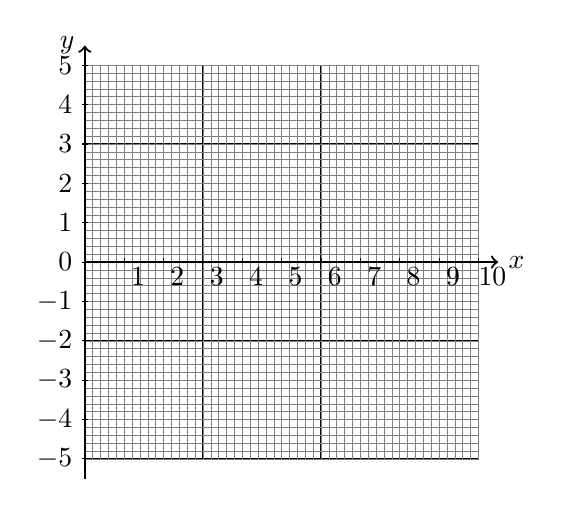
\begin{tikzpicture}[scale=0.5]
    \draw [black, xstep=1.0cm, ystep=1.0cm] (0,-5) grid (10,5);
    \draw [gray, very thin, xstep=0.2cm, ystep=0.2cm] (0,-5) grid (10,5);
    \draw [thick, ->] (0,0) -- (10.5,0) node [right] {$x$};
    \draw [thick, ->] (0,-5.5) -- (0,5.5) node [left] {$y$};    \foreach \x in {1,...,10}
      \draw[shift={(\x,0)}] (0pt,-1pt) -- (0pt,3pt) node[below]{$\quad \x$};
    \foreach \y in {-5,-4,-3,-2,-1,0,1,2,3,4,5}
      \draw[shift={(0,\y)}] (2pt,0pt) -- (-2pt,0pt) node[left]{$\y$};
  \end{tikzpicture}
  \end{center}
\end{figure}


\end{enumerate}
\end{document}
